\section{RT-16 X-joslas raiduztverošās sistēmas pārskats}
Att 1.1. tiek parādīta X-joslas pārskats RT-16 radioteleskopam. Sistēmas vadība tiek veikta ar operatora jeb kontroles datoru, kas vada Cortex modemu \cite{cortex}, frekvenču lejuppārveidotāju un augšuppārveidotāju \cite{up_down_converters}, LNA un HPA. Cortex modēms paredzēts datu modulēšanai un demodulēšanai no satelīta. Frekvenču lejup un augšup pārveidotājs nepieciešams, lai varētu modulēto signālu pārnest uz nepieciešamo nesējfrekvenci noteiktam satelītam. HPA pastiprina modulēto signālu līdz 100 W (+50 dBm), lai palielinātu pārraides attālumu. HPA bloka pārraides jaudu noteica SSC. LNA nepieciešams, lai uzlabotu uztvertā signāla SNR un lai Cortex varētu to veiksmīgi demodulēt. Dipleksers un paraboliskā antena paredzēti signāla uztveršanai un pilna dupleksa komunikācijas nodrošināšanai.
\begin{figure}[H]
	\centering
    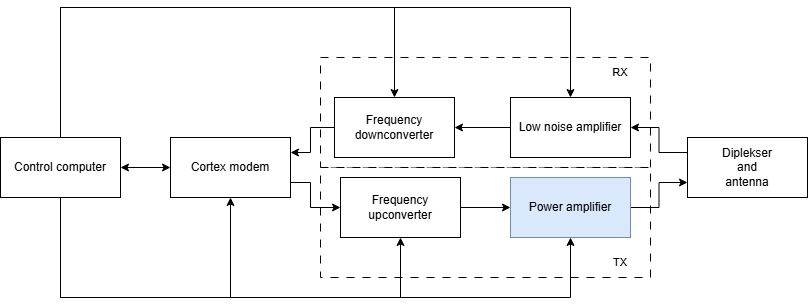
\includegraphics[width=\textwidth]{pictures/rt-16_x_diagram.jpg}\hspace{1cm}
    \caption{RT-16 X-joslas raiduztvērēja vispārīga bloka diagramma}
\end{figure}
Turpmāk darbā tiek apskatīts tikai augstas jaudas pastiprinātājs, kur daļa no tā tiek izstrādāta šī bakalaura ietvaros.